\subsection{Шкала электромагнитных волн}

\term{Гамма излучение} возникает при радиоактивных распадах ядер, при торможении электронов энергией более $10^5$~эВ и при других взаимодействиях элементарных частиц. Используются в гамма-дефектоскопии, при изучении свойств вещества.

\term{Рентгеновские лучи} излучаются при большом ускорении электронов, например при их торможении в металлах. Получают их при помощи рентгеновской трубки: электроны в вакуумной трубке ускоряются электрическим полем при высоком напряжении, достигая анода, при со­ударении резко тормозятся. При торможении электроны движут­ся с ускорением и излучают электромагнитные волны с малой длиной.

\begin{figure}[!h]
	\centering
	\begin{tikzpicture}
        \newcommand{\freqX}[1]{-0.8 - (#1 - 3)/2}
    
        \foreach \f in {3,5,...,19} {
            \tkzDefPoint(\freqX{\f}, 0){F}
            \tkzLabelPoint[below](F){$10^{\f}$}
            \tkzLabelPoint(F){\tiny|}
        }
       
       \tkzDefPoint(0,0){F0}
       \tkzDefPoint(-11.5,0){Fmax}
       \tkzDrawSegment[-latex](F0,Fmax)
       \tkzLabelPoint[above right](Fmax){Частота $\nu$, Гц}
       
       \def\lgC{8.477} 
       \def\Lpos{-0.85}    
       
       \foreach \l in {-12,-10,...,6} {
            \tkzDefPoint(\freqX{\lgC - \l}, \Lpos){L}
            \tkzLabelPoint[below](L){$10^{\l}$}
            \tkzLabelPoint(L){\tiny|}
        }
        
        \tkzDefPoint(0,\Lpos){Lmax}
       \tkzDefPoint(-11.5,\Lpos){L0}
       \tkzDrawSegment[-latex](L0,Lmax)
       \tkzLabelPoint[above right](L0){Длина волны $\lambda$, м}
       
       
       \def\LWmin{3.5}
       \def\LWmax{6.7}
       \tkzDefPoint(\freqX{\lgC - \LWmin}, \Lpos){LW1}
       \tkzDefPoint(\freqX{\lgC - \LWmax}, \Lpos){LW2}
       \tkzDefMidPoint(LW1,LW2) \tkzGetPoint{LW}
       \draw [decorate, decoration = {brace, raise=15pt,  amplitude=5pt}] (LW2) --  (LW1);
       \tkzLabelPoint[below=19pt](LW){\parbox{2cm}{\centering Низкочастотые \\ волны}}
       
        \def\Rmin{-4}
       \def\Rmax{3.5}
       \tkzDefPoint(\freqX{\lgC - \Rmin}, \Lpos){R1}
       \tkzDefPoint(\freqX{\lgC - \Rmax}, \Lpos){R2}
       \tkzDefMidPoint(R1,R2) \tkzGetPoint{R}
       \draw [decorate, decoration = {brace, raise=15pt,  amplitude=5pt}] (R2) --  (R1);
       \tkzLabelPoint[below=19pt](R){Радиоволны}
       
       \def\IRmin{-6.1}
       \def\IRmax{-3}
       \tkzDefPoint(\freqX{\lgC - \IRmin}, \Lpos){IR1}
       \tkzDefPoint(\freqX{\lgC - \IRmax}, \Lpos){IR2}
       \tkzDefMidPoint(IR1,IR2) \tkzGetPoint{IR}
       \draw [decorate, decoration={brace,raise = 20pt, amplitude=3pt}] (IR2) --  (IR1);
       \tkzLabelPoint[below=24pt](IR){ИК}
       
       \def\Vmin{-6.4}
       \def\Vmax{-6.1}
       \tkzDefPoint(\freqX{\lgC - \Vmin}, \Lpos){V1}
       \tkzDefPoint(\freqX{\lgC - \Vmax}, \Lpos){V2}
       \tkzDefMidPoint(V1,V2) \tkzGetPoint{V}

       \draw [decorate, decoration={brace,raise = 20pt, amplitude=1pt}] (V2) --  (V1);
       \tkzDefShiftPoint[V](0,-21pt){V'}
       \tkzDefShiftPoint[V'](0.3,-0.7){V''}
       \tkzDrawSegment(V',V'')
       \tkzLabelPoint[right](V''){Видимый}
       
       \def\UVmin{-8}
       \def\UVmax{-6.4}
       \tkzDefPoint(\freqX{\lgC - \UVmin}, \Lpos){UV1}
       \tkzDefPoint(\freqX{\lgC - \UVmax}, \Lpos){UV2}
       \tkzDefMidPoint(UV1,UV2) \tkzGetPoint{UV}
       \draw [decorate, decoration={brace,raise = 20pt, amplitude=3pt}] (UV2) --  (UV1);
       \tkzLabelPoint[below=24pt](UV){УФ}
       
       \def\Rmin{-12}
       \def\Rmax{-7}
       \tkzDefPoint(\freqX{\lgC - \Rmin}, \Lpos){R1}
       \tkzDefPoint(\freqX{\lgC - \Rmax}, \Lpos){R2}
       \tkzDefMidPoint(R1,R2) \tkzGetPoint{R}
       \draw [decorate, decoration = {brace, raise=15pt,  amplitude=5pt}] (R2) --  (R1);
       \tkzLabelPoint[below=19pt](R){Рентген}
       
       \def\Gmin{-15}
       \def\Gmax{-12}
       \tkzDefPoint(\freqX{\lgC - \Gmin}, \Lpos){G1}
       \tkzDefPoint(\freqX{\lgC - \Gmax}, \Lpos){G2}
       \tkzDefMidPoint(G1,G2) \tkzGetPoint{G}
       \draw [decorate, decoration = {brace, raise=15pt,  amplitude=5pt}] (G2) --  (G1);
       \tkzLabelPoint[below=19pt](G){Гамма}
    \end{tikzpicture}
%	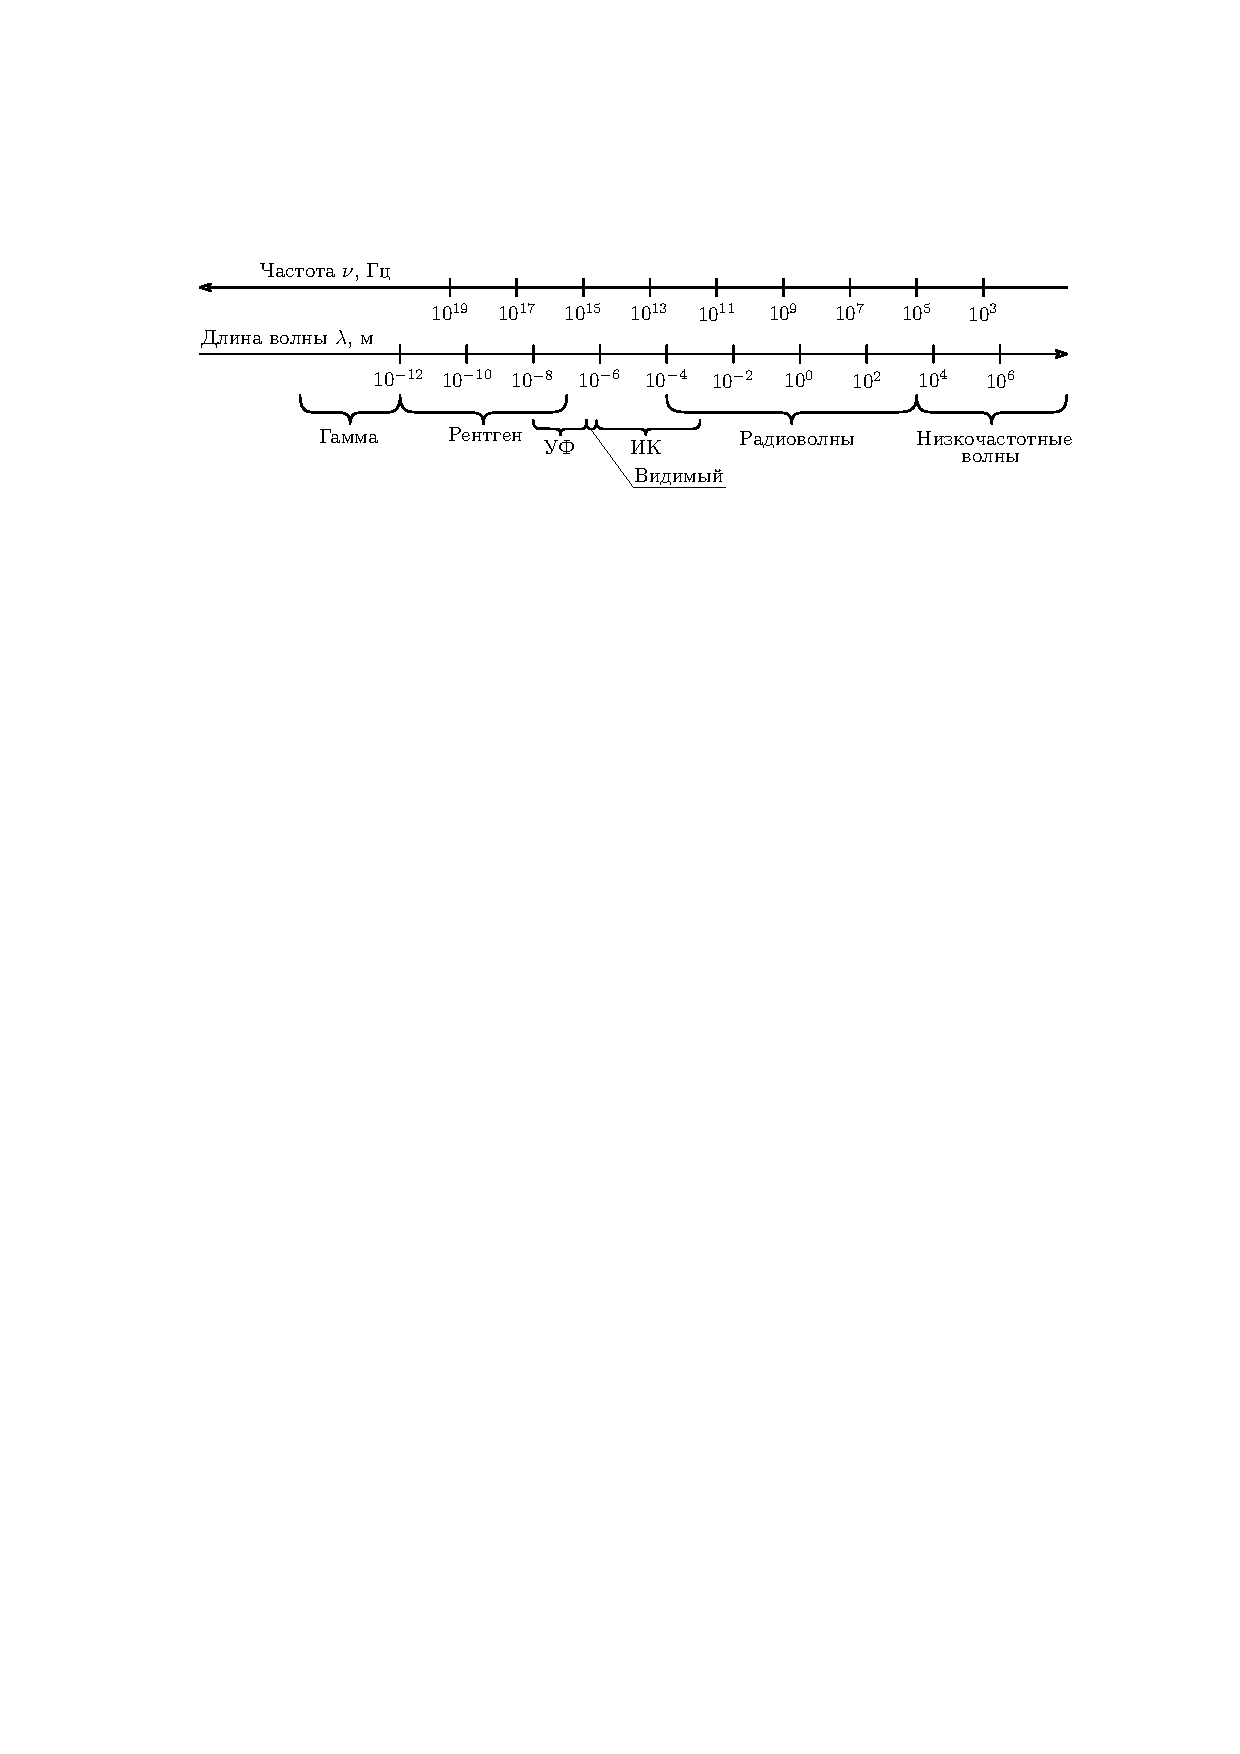
\includegraphics[width = 1\textwidth]{scale-wave.pdf}
	\caption{Шкала электромагнитных волн}
\end{figure}
\term{Ультрафиолетовые лучи}~--- излучение Солнца, ртутных ламп и т.\,п. Используются в ультрафиолетовой микроскопии, в медицине.

\term{Видимое излучение}~--- часть электромагнитного излучения, воспринимаемая глазом (от фиолетового до от красного).

\term{Инфракрасное излучение}~--- тепловое, излучается любым нагретым телом.

\term{Радиоволны} используются повсеместно в обычной жизни, это и сотовая связь, и радиолокация, и спутниковая связь, и Wi-Fi и многое другое.

\term{Низкочастотные волны}~--- диапазон, традиционно используемый в электротехнике. В промышленной электроэнергетике используется частота 50~Гц, на~которой осуществляется передача электрической энергии по линиям и преобразование напряжений трансформаторными устройствами.
